\documentclass[12pt]{article}
%\usepackage[latin1]{inputenc}
\usepackage[T1]{fontenc}
\usepackage{geometry}
\usepackage{graphicx}
\usepackage{subcaption}
\usepackage[onehalfspacing]{setspace}
\usepackage{amsmath,amsfonts,amssymb,amsthm}
\usepackage{bm}
\usepackage{commath}
\usepackage{enumerate}
\usepackage{accents}
%\usepackage{enumitem}
\usepackage[shortlabels]{enumitem}
\usepackage{dsfont}
\usepackage{mathtools}
\usepackage{physics}
\usepackage{cite}
\usepackage[round]{natbib}
\usepackage{caption}
\captionsetup[figure]{font=small}
\usepackage{float}
\usepackage{hyperref}

\newtheorem*{theorem}{Theorem} 
\newtheorem*{lemma}{Lemma}
\newtheorem*{definition}{Definition}
\newtheorem*{corollary}{Corollary}
\newtheorem*{remark}{Remark}
\newtheorem*{example}{Example}
\newtheorem*{examples}{Examples}
\newcommand*{\QEDB}{\hfill\ensuremath{\square}}

\DeclareMathOperator*{\argmax}{arg\,max}
\DeclareMathOperator*{\argmin}{arg\,min}

\newcommand\independent{\protect\mathpalette{\protect\independenT}{\perp}}
\def\independenT#1#2{\mathrel{\rlap{$#1#2$}\mkern2mu{#1#2}}}

\interfootnotelinepenalty=10000
\allowdisplaybreaks
\geometry{
  left=2.5cm,
  right=2.5cm,
  top=2cm,
  bottom=2cm,
}

\graphicspath{{C:/Users/Simon/OneDrive/Uni/LMU/SS 2020/Statistisches Consulting/Bundestag-MP-Analyse/plots/}}

\begin{document}

\section{Results}

\subsection{2-step Approach: CTM}

In sections 4.4 and 4.5, we analyzed the relationship between topic proportions and metadata, visualizing the effect of prevalence covariates and deciding against the further inclusion of a topical content variable. As briefly mentioned in section 2 already, a point of concern when using the STM is the double usage of covariates: they are used in the estimation of the topics themselves (and thus, in the estimation of the latent topic proportions) and subsequently they are again used to estimate their relationship with topic proportions. From classical statistical modeling, we are used to interpret such relationships, oftentimes ascribing a causal interpretation to the corresponding coefficients; in our case, this would go along the lines of stating, for instance, that "a higher percentage of immigrants within an electoral district makes politicians prioritize issues other than climate protection", referring to Figure XXX in section 4.4.1. Topic models, however, present a crucial difference as compared to classical statistical models: the target variable - $\theta$ - is latent and thus itself being estimated. For explorative or descriptive purposes, this does not pose a problem because there is only a single step: discovering topics in the text documents. Yet whenever in a second step, after estimating the model, we wish to conduct (causal) inference, we face an overfitting problem, since the \textit{same} documents and covariates are used in both steps. In this section, we focus on the double usage of (prevalence) covariates, while section 4.7 deals with double usage of documents, i.e., words.

To avoid overfitting due to double usage of covariates, we fit an STM without including any covariates in the model estimation, thus reducing the model to a simple CTM. In a second, isolated step, we estimate the relationship between topic proportions and covariates. That is, we forgo the potential (small) gains of joint estimation of the STM in favor of a clear-cut 2-step procedure which avoids overfitting. As a first step, we fit the CTM analogously to the original STM (which includes topical prevalence variables), the only difference being that no document-level metadata is used in the estimation of the CTM. In line with the performance results in \cite{roberts2016model}, we observe a slightly higher held-out likelihood for the STM (-8.5478) than for the CTM (-8.5492) when holding out a random 50\% of the words from a randomly chosen 10\% of the documents. Moreover, we notice that the topics themselves (in terms of their top words) are almost identical to those of the STM, which is why we use the same topic labeling as in section 4.4. As for differences in topic proportions between the two models on a document level, we consider the average topic proportion deviation per document, $\frac{1}{K}\sum_{k=1}^{K}|\theta_{d,k}(STM)-\theta_{d,k}(CTM)|$. The resulting average difference between topic proportions per topic, averaged across all documents, amounts to 1.61\%; that is, for an average document, the absolute difference in the proportion of each topic is less than 2\%, which is rather moderate. These differences in topic proportions between STM and CTM further cancel each other out across documents: when comparing global topic proportions (i.e., topic proportions simply averaged across all documents), the results are very similar, with the average difference per topic only
amounting to 0.23\%. Altogether, topic proportions seem to be affected by the topical prevalence covariates only to a small degree on an individual document level, and this effect almost disappears entirely if we consider corpus-wide topic proportions.

In the second step, we consider the relationship between topic proportions and prevalence covariates for the CTM and compare the resulting relationships with those of the originally fitted STM (which contains prevalence covariates). For comparability, we use the same methodology as in section 4.4: applying the method of composition with a quasibinomial regression of individual topic proportions on covariates. The only difference is that prevalence covariates were not included in the model used to generate topic proportions. Consequently, sampling all (unnormalized) topic proportions jointly via the logistic normal distribution (as in Figure 4.XXX) is not applicable here, as no $\Gamma$-vector is being estimated at all. In the figures below, we visualize the CTM topic proportions of topics 4 (Social/Housing) and 6 (Climate Protection) in relation with continuous covariate values and across parties and compare the results to those of the STM (Figures XXX and XXX). As for the relationship between continuous covariates and topic proportions, the results for STM and CTM are very similar: for both topic 4 and topic 6, the trends across the respective covariate range are almost identical for the two models, while the scale differs slightly (with scale differences hardly exceeding 2\%). Turning to the categorical variables, in particular party, the conclusion is very similar for topic 4: we observe minor scale differences and very similar patterns. For topic 6, the scale of the topic proportions is again slightly different compared to the STM, and now we also observe some (minor) difference in the relative positioning of the different parties. 

\begin{figure}[h!]
  \centering
  \captionsetup{justification=centering,margin=2cm}
  \begin{subfigure}[b]{0.4\linewidth}
    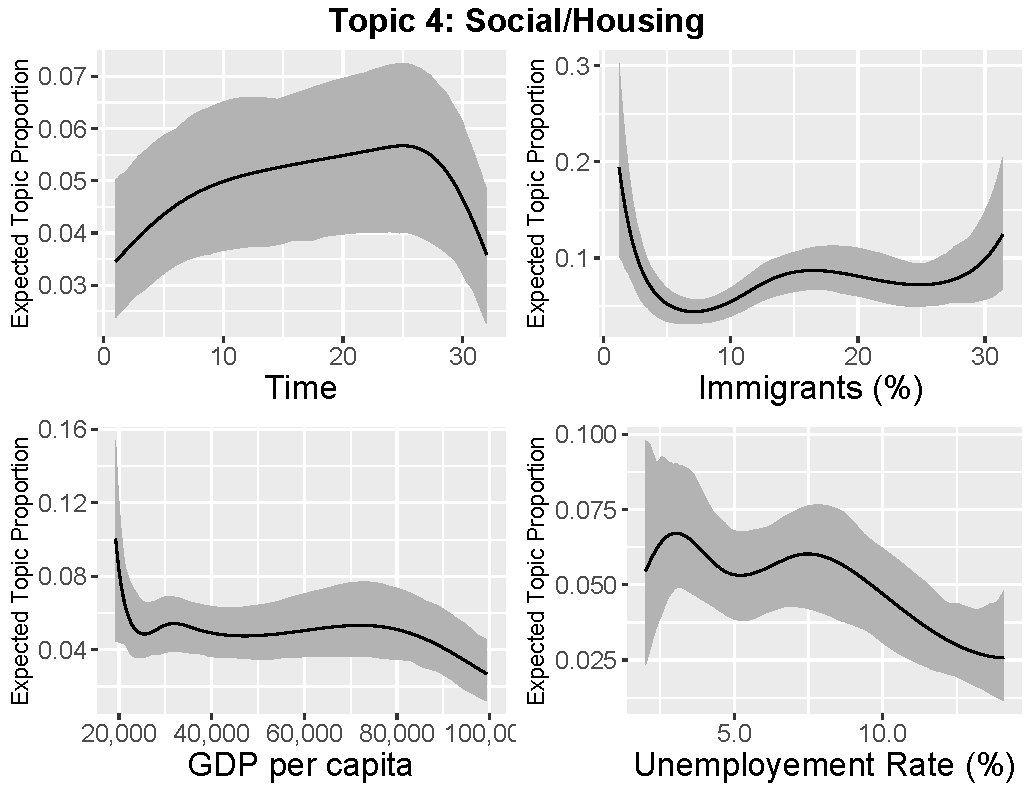
\includegraphics[width=\linewidth]{4_6/quasi_t4_cont_ctm.pdf}
  \end{subfigure}
  \begin{subfigure}[b]{0.4\linewidth}
    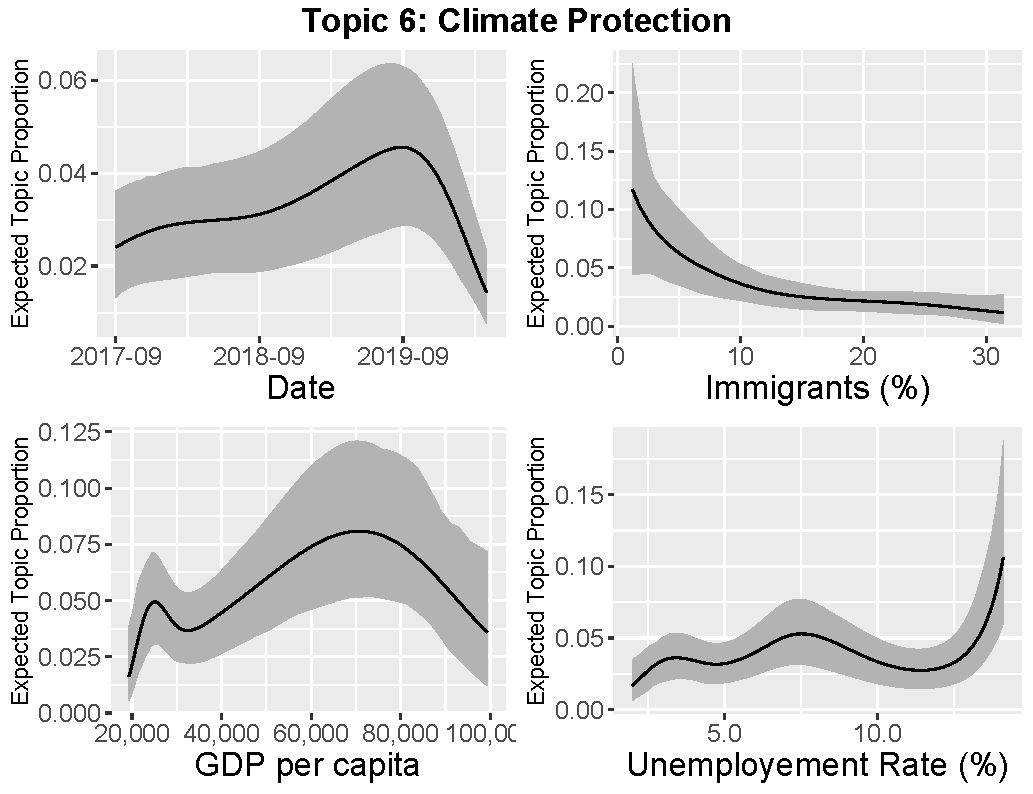
\includegraphics[width=\linewidth]{4_6/quasi_t6_cont_ctm.pdf}
  \end{subfigure}
  \caption{Mean and 95\% credible intervals for smooth effects, obtained
using a quasibinomial GLM (no covariates included in model estimation).}
  \label{fig:quasi_t46_cont_ctm}
\end{figure}

\begin{figure}[h!]
  \centering
  \captionsetup{justification=centering,margin=2cm}
  \begin{subfigure}[b]{0.4\linewidth}
    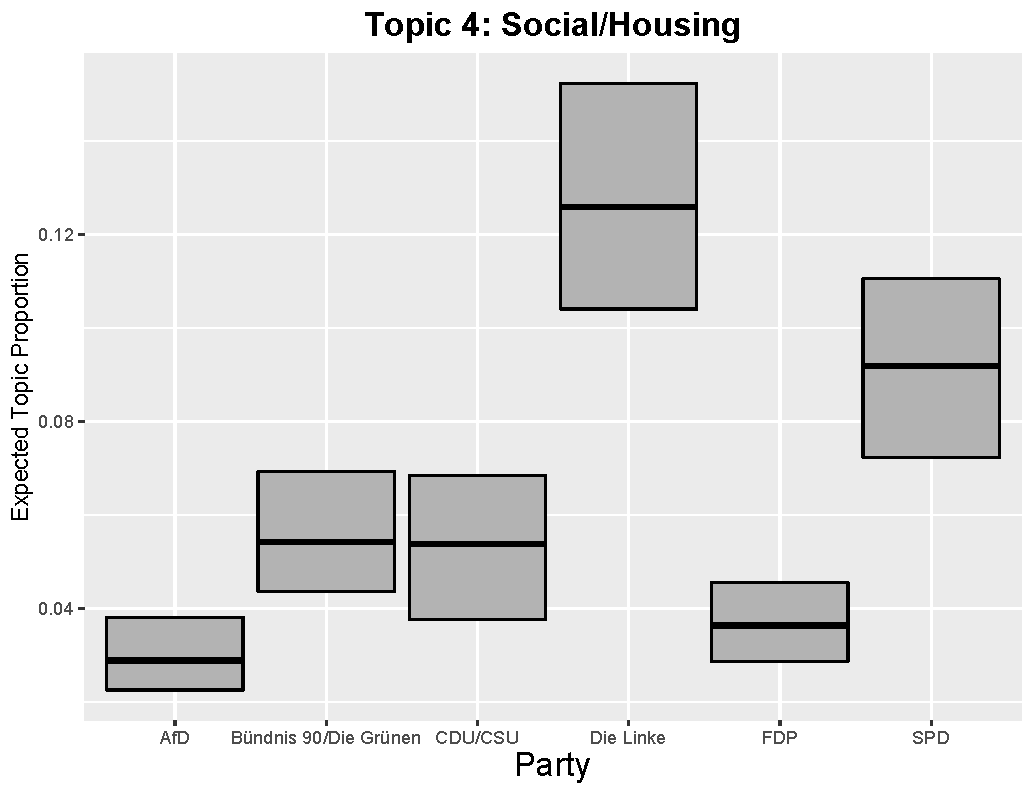
\includegraphics[width=\linewidth]{4_6/quasi_t4_cat_ctm.pdf}
  \end{subfigure}
  \begin{subfigure}[b]{0.4\linewidth}
    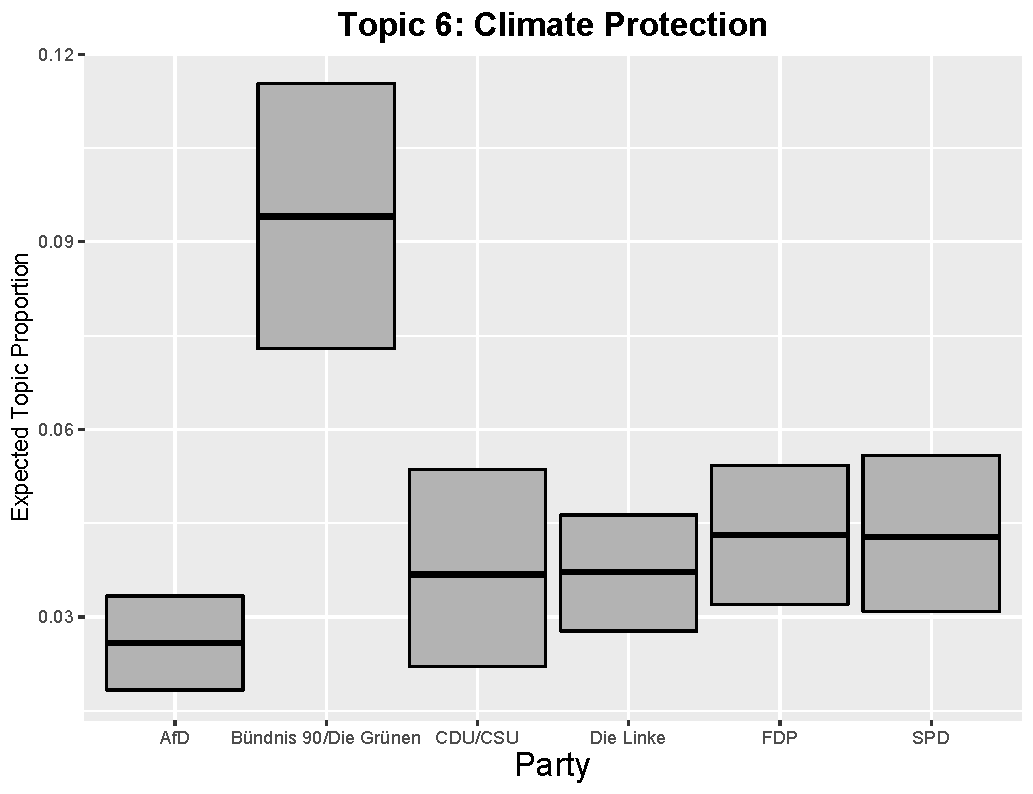
\includegraphics[width=\linewidth]{4_6/quasi_t6_cat_ctm.pdf}
  \end{subfigure}
  \caption{Mean and 95\% credible intervals for different political parties,
obtained using a quasibinomial GLM (no covariates included in model estimation).}
  \label{fig:quasi_t46_cat_ctm}
\end{figure}

Topic proportions across parties for topics 3, 6, and 1 (Right/Nationalist) are further summarized in the plot below. Comparing the results to those of the STM for the additional topic 1, a rather large difference can be seen: the overall topic proportion for the AfD party is now almost 10\% lower than in the STM (though still at almost 35\%). Furthermore, for all topics and covariates, the comparison between STM and CTM does not change if we use Beta regression instead of quasibinomial regression within the method of composition, corroborating our results (see appendix XXX).

\begin{figure}[h!]
  \centering
  \captionsetup{justification=centering,margin=2cm}
  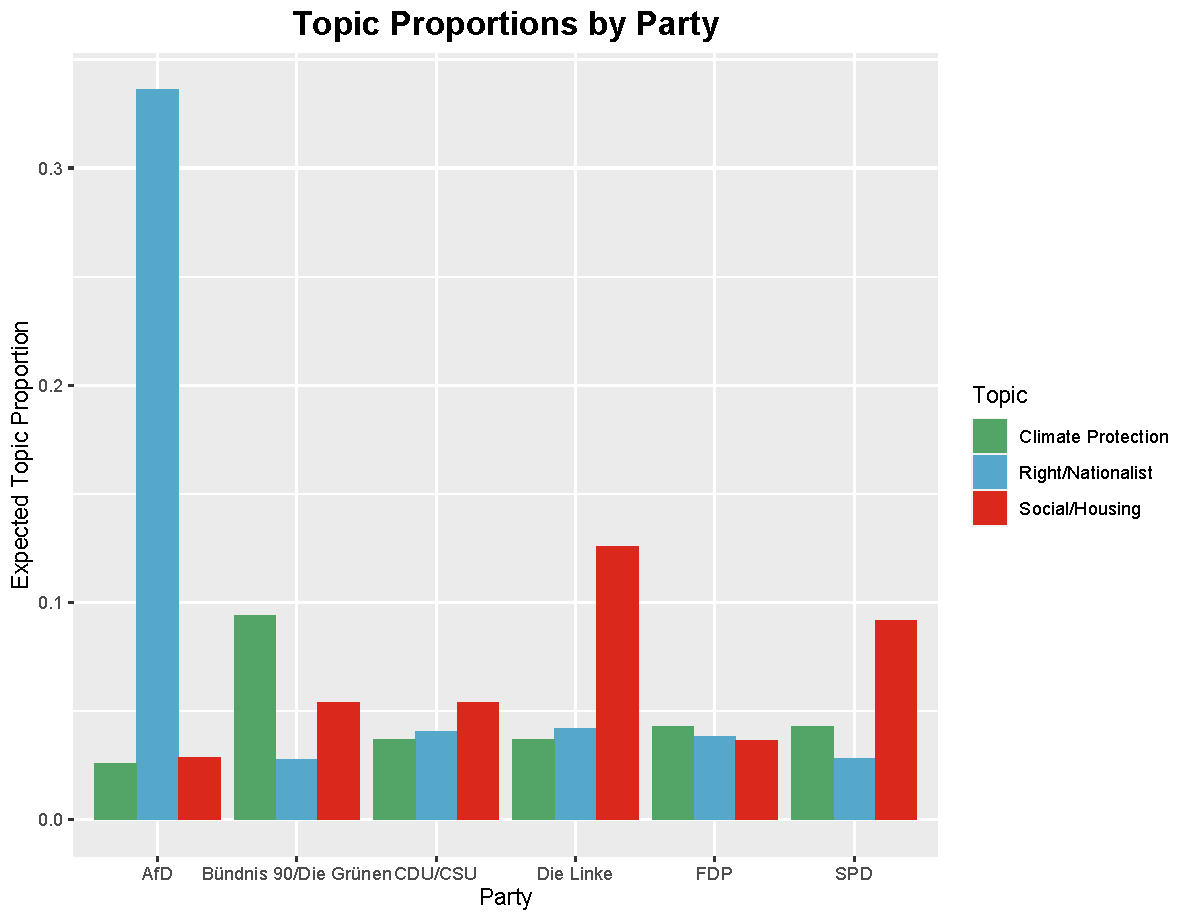
\includegraphics[width=\linewidth]{4_6/quasi_t146_cat_ctm.pdf}
  \caption{Mean and 95\% credible intervals for different political parties,
obtained using a quasibinomial GLM (no covariates included in model estimation).}
  \label{fig:quasi_t146_cat_ctm}
\end{figure}

All in all, the relationships between topical prevalence variables and topic proportions are very similar to those of the STM when instead using a clean 2-step estimation procedure where no covariate information is used in the model estimation. This indicates that the problem of double usage of covariate information in the STM, potentially leading to overfitting, is not overly severe. However, we wish to remind the reader that at this point, we have not yet accounted for the double usage of documents - even in this "clean" 2-step procedure, the estimation of topic proportions is based on the same documents which are associated with the covariate values used in the second step. Section 4.7 finally addresses this open issue.


\bibliography{bibliography}
\bibliographystyle{plainnat}

\end{document}